\documentclass[12pt]{article}
\setlength\parindent{0pt}
\usepackage{amsmath}
\usepackage{lscape}
\usepackage{graphicx}
\usepackage{fullpage}
\usepackage[margin=0.5in]{geometry}
\setlength{\parskip}{4mm}
\def\LL{\left\langle}   % left angle bracket
\def\RR{\right\rangle}  % right angle bracket
\def\LP{\left(}         % left parenthesis
\def\RP{\right)}        % right parenthesis
\def\LB{\left\{}        % left curly bracket
\def\RB{\right\}}       % right curly bracket
\def\PAR#1#2{ {{\partial #1}\over{\partial #2}} }
\def\PARTWO#1#2{ {{\partial^2 #1}\over{\partial #2}^2} }
\def\PARTWOMIX#1#2#3{ {{\partial^2 #1}\over{\partial #2 \partial #3}} }
\newcommand{\BE}{\begin{displaymath}}
\newcommand{\BC}{\begin{center}}
\newcommand{\EC}{\end{center}}
\newcommand{\EE}{\end{displaymath}}
\newcommand{\BNE}{\begin{equation}}
\newcommand{\ENE}{\end{equation}}
\newcommand{\BEA}{\begin{eqnarray}}
\newcommand{\EEA}{\nonumber\end{eqnarray}}
\newcommand{\EL}{\nonumber\\}
\newcommand{\la}[1]{\label{#1}}
\newcommand{\ie}{{\em i.e.\ }}
\newcommand{\eg}{{\em e.\,g.\ }}
\newcommand{\cf}{cf.\ }
\newcommand{\etc}{etc.\ }
\newcommand{\Tr}{{\rm tr}}
\newcommand{\etal}{{\it et al.}}
\newcommand{\OL}[1]{\overline{#1}\ } % overline
\newcommand{\OLL}[1]{\overline{\overline{#1}}\ } % double overline
\newcommand{\OON}{\frac{1}{N}} % "one over N"
\newcommand{\OOX}[1]{\frac{1}{#1}} % "one over X"
\pagenumbering{gobble}
\begin{document}
\Large
\centerline{\sc{Quiz 5 - Spectroscopy (form B)}}

\vspace{1em}


\begin{minipage}{0.6\textwidth}
	Name: \underline{\hspace{3in}}
\end{minipage}
\begin{minipage}{0.4\textwidth}
	\Large
	Lab Section: M0\underline{\hspace{1in}}\\
	\small (if you want your paper back)
\end{minipage}


\normalsize

	\rm
	
	\begin{enumerate}
		\item Suppose an element has four energy levels of 0 eV, 2.3 eV, 3.9 eV, and  5 eV. 
		
		\begin{enumerate}
			\item Draw an energy level diagram for this element below.
			
			\vspace{4in}
			
			\item Indicate what spectral lines you would see with your eye if you ran electric current through a diffuse gas of this element.
			
			\begin{minipage}{\textwidth}

				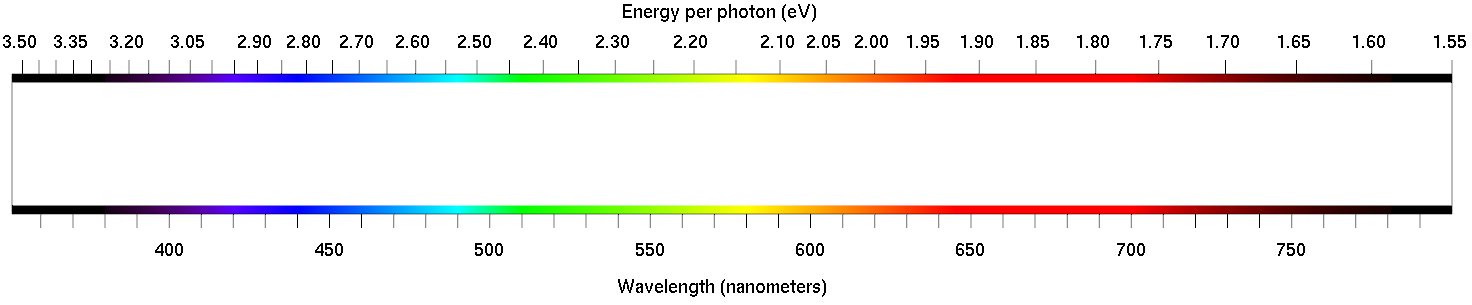
\includegraphics[width=5.5in]{spectrum-blank.png}

			\end{minipage}
			
			\item Would there be any other photon energies emitted that you cannot see? If so, what are they?
		\end{enumerate}
	
	\newpage
	
	\item Astronomers observe a Sunlike star that contains only hydrogen and helium using a space telescope (so there is no interference from Earth).
	
    \begin{enumerate} 
    	\item What sort of spectrum would they see? Specifically, would they see a continuous band of color, a few thin bright lines, or a continuous band of color with dark lines on top of it?
    	
    	\vspace{2in}
    	
    	\item Suppose that now a planet with a thick nitrogen atmosphere passes in front of the star, so that the starlight must also pass through the planet's atmosphere. Describe how its spectrum would change. Would a continuous band of color appear or change? Would dark or bright lines appear or disappear? Explain briefly why this would happen.
    	
    	\vspace{2in}
    \end{enumerate}
		\item Describe in a few sentences, in your own words, how the dark lines in the Sun's spectrum tell us what the Sun is made of.
	
	\vspace{3in}
	

	
	\end{enumerate}
	
	
 
\end{document}

